\chapter{Klaidinanti Opera Mini mygtuko antraštė}

\section{Tikslas}

Parsisiųsti failą iš interneto, naudojant mobilųjį telefoną.

\section{Priemonės}

\ref{fig:case_2} paveiksluose pateikta naršyklės pateikiamų dialogų
seka, kai yra bandoma parsisiųsti failą. Paskutiniame dialoge
(\ref{fig:case_2_final_dialog}) tampa neaišku kas atsitiko: parašyta,
jog „Atsiuntimas baigtas“, bet tuo pačiu tėra vienintelis
pasirinkimas „Atsisakyti“ ir jis yra virš dešiniojo funkcinio
mygtuko (virš kairiojo mygtuko paprastai būna pasirinkimai tokie,
kaip „Gerai“, „Ok“, „Taip“, o virš dešiniojo „Atšaukti“,
„Ne“ ir „Išeiti“).

\begin{figure}[H]
  \centering
  \subfloat[Failo išsaugojimas]{%
    \label{fig:case_2_save_dialog}%
    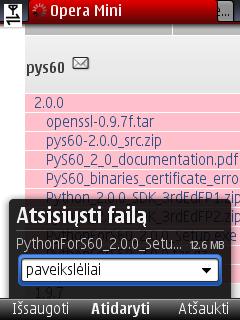
\includegraphics[width=0.3\textwidth]{images/case_2_save_dialog.png}}                
  \subfloat[Siunčiama]{%
    \label{fig:case_2_in_progress}%
    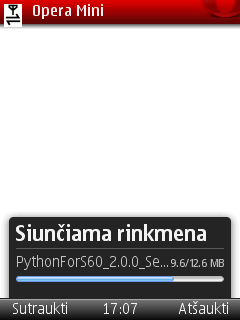
\includegraphics[width=0.3\textwidth]{images/case_2_in_progress.png}}
  \subfloat[Failas parsiųstas]{%
    \label{fig:case_2_final_dialog}%
    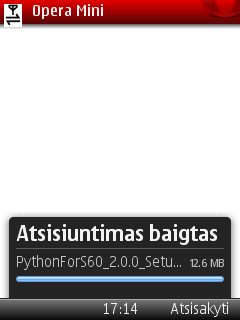
\includegraphics[width=0.3\textwidth]{images/case_2_final_dialog.png}}
  \caption{Failo parsisiuntimas Opera Mini naršyklėje}
  \label{fig:case_2}
\end{figure}

\subsection{Rezultatas}

Pasirinkus vienintelį galima pasirinkimą „Atsisakyti“ ir paskui patikrinus
atsisiųstąjį failą, paaiškėjo, kad su juo viskas yra gerai.

\subsection{Panaudojamumo principas}

Šiame pavyzdyje buvo pažeistas nuspėjamumo principas: buvo neaišku kas
atsitiks nuspaudus vienintelį galimą mygtuką. Taip pat buvo pažeistas
ir darnos principas: kadangi failo atsiuntimas pavyko, tai apie tai
pranešančio dialogo uždarymui neturėtų būti naudojamas tas pats
mygtukas, kuris įprastai yra skirtas operacijų atšaukimui.

\subsection{Pamąstymai}

Greičiausiai, šis pranešimas yra tiesiog programavimo klaida: mygtukui
nurodytas neteisingas tipas.
